%***********************************
\begin{frame}{Learning Objectives}
%***********************************
By the end of this chapter, you will be able to:
\begin{itemize}
\item Understand the fundamentals of Boolean algebra and its applications
\item Construct and analyze truth tables for logical operations
\item Design and optimize combinational logic circuits
\item Apply Boolean laws and identities for circuit simplification
\item Understand the relationship between mathematical logic and digital circuits
\item Recognize the historical development of Boolean algebra in computing
\end{itemize}
\end{frame}

% subsection 1: Introduction to 0-OS
\subsection{Introduction to Zero-Order Systems}

%**************************************************
\begin{frame}{What are Zero-Order Systems (0-OS)?}
%***************************************************
\begin{itemize}
\item \concept{Definition}: Digital systems with \textbf{no feedback loops}
\begin{itemize}
\item Output depends \textit{only} on current input values
\item No memory or state retention
\item Purely combinational behavior
\end{itemize}
\vspace{0.5cm}
\item \concept{Characteristics}:
\begin{itemize}
\item Immediate response to input changes
\item No temporal dependencies
\item Foundation for all digital logic
\item Building blocks for higher-order systems
\end{itemize}
\vspace{0.3cm}
\item \concept{Examples}: Logic gates, decoders, multiplexers, adders
\end{itemize}
\end{frame}

%*******************************************
\begin{frame}{Order-Based System Hierarchy}
%********************************************
\begin{itemize}
\item \concept{0-OS (Zero-Order)}: Combinational circuits
\begin{itemize}
\item No loops, no memory
\item Output = f(current inputs)
\end{itemize}
\vspace{0.3cm}
\item \concept{1-OS (First-Order)}: Memory circuits
\begin{itemize}
\item One feedback loop
\item Can store state
\end{itemize}
\vspace{0.3cm}
\item \concept{2-OS (Second-Order)}: Automata
\begin{itemize}
\item Two feedback loops
\item Autonomous behavior
\end{itemize}
\vspace{0.3cm}
\item \concept{3-OS (Third-Order)}: Processors
\begin{itemize}
\item Three feedback loops
\item Complex computational behavior
\end{itemize}
\end{itemize}
\end{frame}

% subsection 2: Boolean Algebra
\subsection{Boolean Algebra}

%**************************************
\begin{frame}{Historical Background}
%**************************************
\begin{itemize}
\item \concept{George Boole (1815-1864)}:
\begin{itemize}
\item Published "An Investigation of the Laws of Thought" (1854)
\item Formalized logical reasoning using algebraic structures
\item Created symbolic language for logic
\end{itemize}
\vspace{0.5cm}
\item \concept{Claude Shannon (1916-2001)}:
\begin{itemize}
\item Master's thesis: "A Symbolic Analysis of Relay and Switching Circuits" (1938)
\item Connected Boolean algebra to electrical circuits
\item Foundation of digital circuit design
\item Enabled modern computer development
\end{itemize}
\vspace{0.3cm}
\item \concept{Impact}: Transformed abstract mathematics into practical engineering tool
\end{itemize}
\end{frame}

%*********************************************
\begin{frame}{Boolean Algebra Fundamentals}
%*********************************************
\begin{itemize}
\item \concept{Binary Set}: $B = \{0, 1\}$
\begin{itemize}
\item $0$ represents \textbf{false}
\item $1$ represents \textbf{true}
\end{itemize}
\vspace{0.5cm}
\item \concept{Basic Operations}:
\begin{itemize}
\item \textbf{AND} ($\land$): $A \land B = 1$ iff both $A = 1$ and $B = 1$
\item \textbf{OR} ($\lor$): $A \lor B = 1$ if at least one of $A$ or $B$ equals $1$
\item \textbf{NOT} ($\neg$): $\neg A = 1$ if $A = 0$, and $\neg A = 0$ if $A = 1$
\end{itemize}
\vspace{0.3cm}
\item \concept{Physical Interpretation}:
\begin{itemize}
\item $0$ = Low voltage, switch open, false
\item $1$ = High voltage, switch closed, true
\end{itemize}
\end{itemize}
\end{frame}

%******************************************
\begin{frame}{Boolean Laws and Identities}
%******************************************
\begin{columns}
\begin{column}{0.5\textwidth}
\concept{Commutative Laws}:
\begin{align}
A \lor B &= B \lor A\\
A \land B &= B \land A
\end{align}

\concept{Associative Laws}:
\begin{align}
A \lor (B \lor C) &= (A \lor B) \lor C\\
A \land (B \land C) &= (A \land B) \land C
\end{align}

\concept{Distributive Laws}:
\begin{align}
A \land (B \lor C) &= (A \land B) \lor (A \land C)\\
A \lor (B \land C) &= (A \lor B) \land (A \lor C)
\end{align}
\end{column}
\begin{column}{0.5\textwidth}
\concept{Identity Laws}:
\begin{align}
A \lor 0 &= A\\
A \land 1 &= A
\end{align}

\concept{Complement Laws}:
\begin{align}
A \lor \neg A &= 1\\
A \land \neg A &= 0
\end{align}

\concept{De Morgan's Laws}:
\begin{align}
\neg(A \lor B) &= \neg A \land \neg B\\
\neg(A \land B) &= \neg A \lor \neg B
\end{align}
\end{column}
\end{columns}
\end{frame}

%********************************************
\begin{frame}{Boolean Algebra Applications}
%*******************************************
\begin{itemize}
\item \concept{Circuit Simplification}:
\begin{itemize}
\item Reduce number of gates required
\item Minimize cost and complexity
\item Improve performance and reliability
\end{itemize}
\vspace{0.5cm}
\item \concept{Simplification Methods}:
\begin{itemize}
\item \textbf{Boolean identities}: Algebraic manipulation
\item \textbf{Karnaugh maps}: Graphical simplification method
\item \textbf{Quine-McCluskey algorithm}: Tabular minimization approach
\end{itemize}
\vspace{0.5cm}
\item \concept{Logic Conversion}:
\begin{itemize}
\item Convert between AND-OR and NAND-NOR logic
\item Transform to preferred gate types
\item Optimize for specific technologies
\end{itemize}
\end{itemize}
\end{frame}

% subsection 3: Truth Tables
\subsection{Truth Tables}

%****************************************
\begin{frame}{Truth Table Fundamentals}
%*****************************************
\begin{itemize}
\item \concept{Definition}: Systematic representation of logical expressions
\begin{itemize}
\item Lists all possible input combinations
\item Shows corresponding output values
\item Complete behavioral specification
\end{itemize}
\vspace{0.5cm}
\item \concept{Structure Components}:
\begin{itemize}
\item \textbf{Input Variables}: Columns for logical variables ($A, B, \ldots, N$)
\item \textbf{Output Values}: Results of logical operations
\item \textbf{Rows}: $2^n$ combinations for $n$ variables
\end{itemize}
\vspace{0.3cm}
\item \concept{Applications}:
\begin{itemize}
\item Circuit analysis and design
\item Logic verification
\item Boolean function specification
\end{itemize}
\end{itemize}
\end{frame}

%********************************************
\begin{frame}{Basic Logic Operations - Truth Tables}
%********************************************
\begin{columns}
\begin{column}{0.25\textwidth}
\concept{NOT Operation}:
\[
\begin{array}{|c|c|}
\hline
A & \neg A \\
\hline
0 & 1 \\
1 & 0 \\
\hline
\end{array}
\]
\end{column}
\begin{column}{0.35\textwidth}
\concept{AND Operation}:
\[
\begin{array}{|c|c|c|}
\hline
A & B & A \land B \\
\hline
0 & 0 & 0 \\
0 & 1 & 0 \\
1 & 0 & 0 \\
1 & 1 & 1 \\
\hline
\end{array}
\]
\end{column}
\begin{column}{0.35\textwidth}
\concept{OR Operation}:
\[
\begin{array}{|c|c|c|}
\hline
A & B & A \lor B \\
\hline
0 & 0 & 0 \\
0 & 1 & 1 \\
1 & 0 & 1 \\
1 & 1 & 1 \\
\hline
\end{array}
\]
\end{column}
\end{columns}

\vspace{0.5cm}
\begin{columns}
\begin{column}{0.5\textwidth}
\concept{XOR (Exclusive OR)}:
\[
\begin{array}{|c|c|c|}
\hline
A & B & A \oplus B \\
\hline
0 & 0 & 0 \\
0 & 1 & 1 \\
1 & 0 & 1 \\
1 & 1 & 0 \\
\hline
\end{array}
\]
\end{column}
\begin{column}{0.5\textwidth}
\concept{NAND (NOT AND)}:
\[
\begin{array}{|c|c|c|}
\hline
A & B & \neg(A \land B) \\
\hline
0 & 0 & 1 \\
0 & 1 & 1 \\
1 & 0 & 1 \\
1 & 1 & 0 \\
\hline
\end{array}
\]
\end{column}
\end{columns}
\end{frame}

%********************************************
\begin{frame}{Additional Logic Operations}
%********************************************
\begin{columns}
\begin{column}{0.5\textwidth}
\concept{NOR (NOT OR)}:
\[
\begin{array}{|c|c|c|}
\hline
A & B & \neg(A \lor B) \\
\hline
0 & 0 & 1 \\
0 & 1 & 0 \\
1 & 0 & 0 \\
1 & 1 & 0 \\
\hline
\end{array}
\]
\end{column}
\begin{column}{0.5\textwidth}
\concept{XNOR (Equivalence)}:
\[
\begin{array}{|c|c|c|}
\hline
A & B & A \odot B \\
\hline
0 & 0 & 1 \\
0 & 1 & 0 \\
1 & 0 & 0 \\
1 & 1 & 1 \\
\hline
\end{array}
\]
\end{column}
\end{columns}

\vspace{0.5cm}
\concept{Key Properties}:
\begin{itemize}
\item \textbf{NAND}: Universal gate (can implement any Boolean function)
\item \textbf{NOR}: Also universal gate
\item \textbf{XOR}: Useful for parity checking and arithmetic
\item \textbf{XNOR}: Equivalence testing and error detection
\end{itemize}
\end{frame}

\begin{frame}{Truth Table Applications}
\begin{itemize}
\item \concept{Circuit Analysis}:
\begin{itemize}
\item Verify circuit behavior
\item Compare expected vs. actual outputs
\item Debug logic errors
\end{itemize}
\vspace{0.5cm}
\item \concept{Function Specification}:
\begin{itemize}
\item Define required circuit behavior
\item Specify input-output relationships
\item Document design requirements
\end{itemize}
\vspace{0.5cm}
\item \concept{Logic Synthesis}:
\begin{itemize}
\item Convert truth tables to Boolean expressions
\item Generate minimal circuit implementations
\item Optimize for area, speed, or power
\end{itemize}
\end{itemize}
\end{frame}

% subsection 4: Logic Gates and Circuits
\subsection{Logic Gates and Digital Circuits}

%********************************************
\begin{frame}{Logic Gates Summary}
%********************************************
\begin{columns}
\begin{column}{0.65\textwidth}
\renewcommand{\arraystretch}{1.2} % Adjust row height
\setlength{\tabcolsep}{3pt} % Adjust column spacing
\begin{table}
%\centering
\raggedright
\scriptsize % Make text smaller to fit
\begin{tabular}{|>{\centering\arraybackslash}p{1.5cm}|>{\centering\arraybackslash}p{2.2cm}|>{\centering\arraybackslash}p{1.2cm}|>{\centering\arraybackslash}p{3cm}|}
\hline
\textbf{Logic Gate} & \textbf{Numerical} & \textbf{Symbolic} & \textbf{Alternative Names} \\ \hline

OR  & Logical addition \( A + B \) & \( A \lor B \) & Disjunction, Inclusive OR \\ \hline

NOR  & Complement of OR: \( 1 - (A + B) \) & \( \neg (A \lor B) \) & Peirce Arrow, Universal Gate \\ \hline

AND & Logical multiplication \( A \cdot B \) & \( A \land B \) & Conjunction, Multiply Gate \\ \hline

NAND  & Complement of AND: \( 1 - (A \cdot B) \) & \( \neg (A \land B) \) & Sheffer Stroke, Universal Gate \\ \hline

XOR  & Modulo-2 addition \( A \oplus B \) & \( A \oplus B \) & Exclusive OR, Anticoincidence \\ \hline

XNOR  & Complement of XOR: \( 1 - (A \oplus B) \) & \( \neg (A \oplus B) \) & Equality Gate, Coincidence \\ \hline

\end{tabular}
\caption{Summary of Logical Gates and their Interpretations}
\end{table}
\end{column}
\begin{column}{0.4\textwidth}
\scalebox{0.8}{\input{figures/02_07_two_input_gates.lp}}
%\placedrawing[H]{figures/02_07_two_input_gates.lp}{Graphical representation of the most used two-input gates.}{fig:graphical_gates}
\end{column}
\end{columns}
\end{frame}

%*****************************************************
\begin{frame}{Physical Implementation of Logic Gates}
%******************************************************
\begin{columns}[T,totalwidth=\textwidth]
% ==== Left column: bullets ====
\begin{column}{0.7\textwidth}
\begin{itemize}
\item \concept{Transistor-Level Implementation}:
\begin{itemize}
\item CMOS technology (Complementary Metal-Oxide-Semiconductor)
\item NMOS and PMOS transistors
\item Low power consumption and high noise immunity
\end{itemize}

\vspace{0.3cm}

\item \concept{Gate Characteristics}:
\begin{itemize}
\item \textbf{Propagation delay}: Time for output to respond to input change
\item \textbf{Fan-in}: Number of inputs a gate can accept
\item \textbf{Fan-out}: Number of gates an output can drive
\item \textbf{Noise margin}: Tolerance to signal variations
\end{itemize}

\vspace{0.3cm}

\item \concept{Performance Considerations}:
\begin{itemize}
\item Speed vs. power trade-offs
\item Area optimization
\item Signal integrity
\end{itemize}
\end{itemize}
\end{column}

% ==== Right column: LP drawing ====
\begin{column}{0.3\textwidth}
\hspace*{-0.3cm} % shift left slightly if needed
\scalebox{0.6}{\input{figures/02_08_non_inverting_gate_waveforms.lp}}
% Or if you prefer using your custom macro:
% \placedrawing[H]{figures/02_08_non_inverting_gate_waveforms.lp}{Waveforms for the non-inverting gates.}{fig:waveforms}
\end{column}

\end{columns}
\end{frame}

%******************************************************
% \begin{frame}{Combinational Circuit Design Process}
%*******************************************************
% \begin{enumerate}
% \item \concept{Problem Specification}:
% \begin{itemize}
% \item Define input and output requirements
% \item Specify functional behavior
% \item Identify constraints (timing, power, area)
% \end{itemize}
% \vspace{0.3cm}
% \item \concept{Truth Table Construction}:
% \begin{itemize}
% \item List all input combinations
% \item Determine corresponding outputs
% \item Verify completeness and correctness
% \end{itemize}
% \vspace{0.3cm}
% \item \concept{Boolean Expression Derivation}:
% \begin{itemize}
% \item Sum-of-products (SOP) form
% \item Product-of-sums (POS) form
% \item Choose optimal representation
% \end{itemize}
% \vspace{0.3cm}
% \item \concept{Circuit Implementation}:
% \begin{itemize}
% \item Select appropriate gates
% \item Optimize for design goals
% \item Verify functionality
% \end{itemize}
% \end{enumerate}
% \end{frame}


% subsection 5: Combinational Building Blocks
\subsection{Combinational Building Blocks}

%********************************************
\begin{frame}{Decoders}
%********************************************
\begin{columns}[T,totalwidth=\textwidth]

  % ----- Left: bullets -----
  \begin{column}{0.62\textwidth}
    \begin{itemize}
      \item \concept{Function}: Convert binary code to one-hot output
        \begin{itemize}
          \item $n$ inputs produce $2^n$ outputs
          \item Only one output is active (high) at a time
          \item Used for address decoding and selection
        \end{itemize}
      \vspace{0.2cm}
      \item \concept{Applications}:
        \begin{itemize}
          \item Memory address decoding
          \item Instruction decoding in processors
          \item Device selection in systems
          \item Seven-segment display drivers
        \end{itemize}
    \end{itemize}
  \end{column}

  % ----- Right: image + truth table -----
  \begin{column}{0.35\textwidth}
  \concept{2-to-4 Decoder}
    \centering
    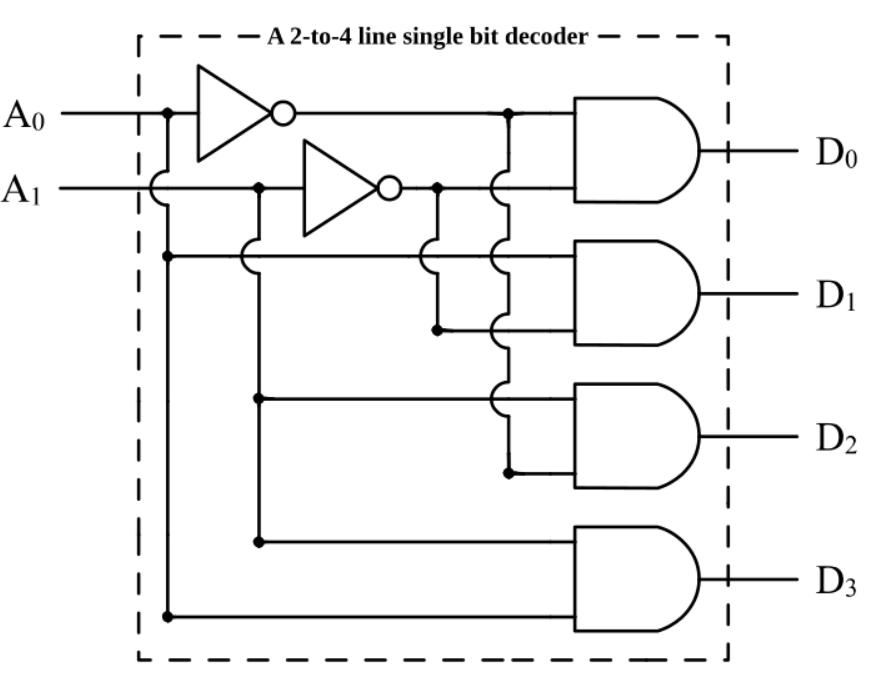
\includegraphics[width=\linewidth]{Latex/Images/2_to_4_decoder.png}

    \vspace{0.6em}

    {\scriptsize
    \setlength{\tabcolsep}{6pt}%
    \renewcommand{\arraystretch}{1.15}%
    \scalebox{0.85}{%
      \begin{tabular}{cc|cccc}
        \toprule
        $A_1$ & $A_0$ & $Y_0$ & $Y_1$ & $Y_2$ & $Y_3$ \\
        \midrule
        0 & 0 & 1 & 0 & 0 & 0 \\
        0 & 1 & 0 & 1 & 0 & 0 \\
        1 & 0 & 0 & 0 & 1 & 0 \\
        1 & 1 & 0 & 0 & 0 & 1 \\
        \bottomrule
      \end{tabular}%
    }}
  \end{column}

\end{columns}
\end{frame}


%********************************************
\begin{frame}{Multiplexers (Data Selectors)}
%********************************************
\begin{columns}[T,totalwidth=\textwidth]

  % ----- Left: bullets -----
  \begin{column}{0.62\textwidth}
    \begin{itemize}
      \item \concept{Function}: Select one of multiple inputs based on control signals
        \begin{itemize}
          \item $2^n$ data inputs, $n$ select inputs
          \item One output that equals the selected input
          \item Digital equivalent of a rotary switch
        \end{itemize}
      \vspace{0.5cm}

      \item \concept{Applications}:
        \begin{itemize}
          \item Data routing and switching
          \item Function generation
          \item Parallel-to-serial conversion
          \item Processor data paths
        \end{itemize}
    \end{itemize}
  \end{column}

  % ----- Right: figure + truth table -----
  \begin{column}{0.35\textwidth}
  \concept{4-to-1 Multiplexor}
  \vspace{0.2cm}
    \centering
    
    
    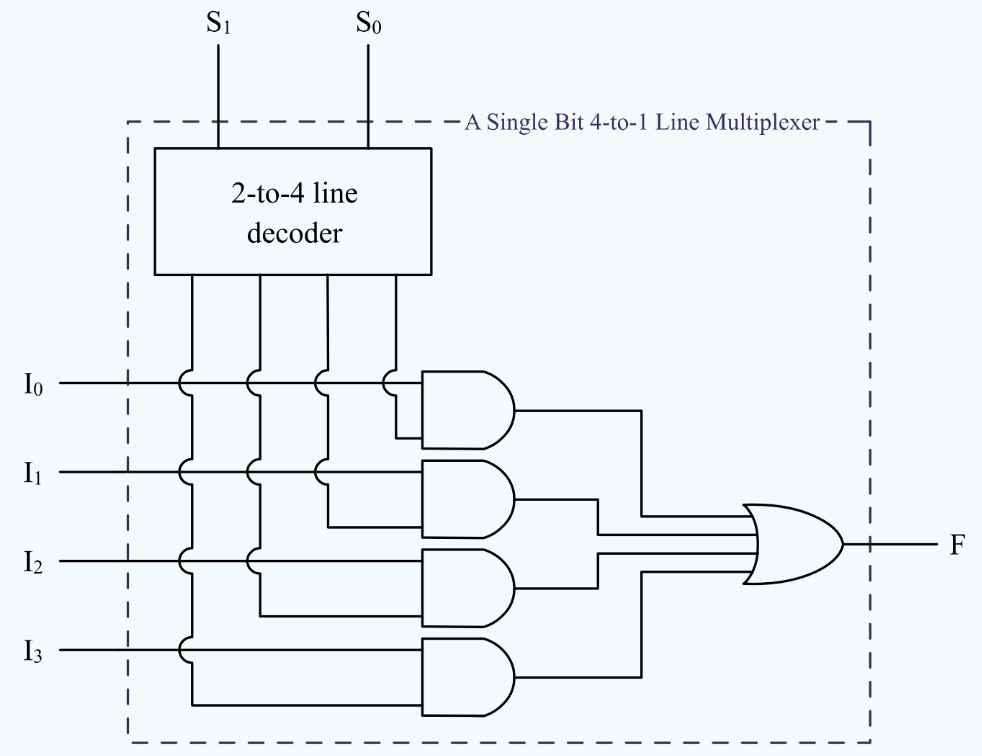
\includegraphics[width=\linewidth]{Latex/Images/4_to_1_mux.png}

    \vspace{0.6em}

    {\scriptsize
    \setlength{\tabcolsep}{6pt}%
    \renewcommand{\arraystretch}{1.15}%
    \scalebox{0.9}{%
      \begin{tabular}{cc|c}
        \toprule
        $S_1$ & $S_0$ & $Y$ \\
        \midrule
        0 & 0 & $I_0$ \\
        0 & 1 & $I_1$ \\
        1 & 0 & $I_2$ \\
        1 & 1 & $I_3$ \\
        \bottomrule
      \end{tabular}%
    }}\\[-2pt]

  \end{column}

\end{columns}
\end{frame}

%**************************************************
\begin{frame}{Demultiplexers (Data Distributors)}
%**************************************************
\begin{columns}[T,totalwidth=\textwidth]

  % ----- Left: bullets -----
  \begin{column}{0.62\textwidth}
    \begin{itemize}
      \item \concept{Function}: Route single input to one of multiple outputs
        \begin{itemize}
          \item One data input, $n$ select inputs
          \item $2^n$ outputs; only one receives data
          \item Inverse operation of a multiplexer
        \end{itemize}
      \vspace{0.5cm}

      \item \concept{Applications}:
        \begin{itemize}
          \item Data distribution
          \item Serial-to-parallel conversion
          \item Address decoding with enable
          \item Communication systems
        \end{itemize}
    \end{itemize}
  \end{column}

  % ----- Right: figure + truth table -----
  \begin{column}{0.35\textwidth}
  \concept{1-to-4 Demultiplexer}
    \centering
    % Update path/filename if needed:
    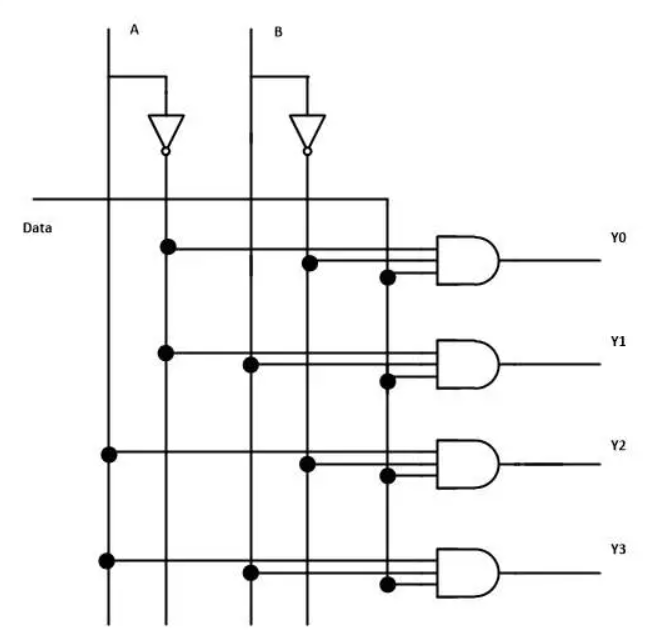
\includegraphics[width=.9\linewidth]{Latex/Images/1_to_4_demux.png}

    \vspace{0.6em}

    {\scriptsize
      \setlength{\tabcolsep}{6pt}%
      \renewcommand{\arraystretch}{1.12}%
      \begin{tabular}{cc|c|cccc}
        \toprule
        $A$ & $B$ & $D$ & $Y_0$ & $Y_1$ & $Y_2$ & $Y_3$ \\
        \midrule
        0 & 0 & $D$ & $D$ & 0   & 0   & 0   \\
        0 & 1 & $D$ & 0   & $D$ & 0   & 0   \\
        1 & 0 & $D$ & 0   & 0   & $D$ & 0   \\
        1 & 1 & $D$ & 0   & 0   & 0   & $D$ \\
        \bottomrule
      \end{tabular}
    }

  \end{column}

\end{columns}
\end{frame}

% %***********************************
% \begin{frame}{Encoders}
% %************************************
% \begin{itemize}
% \item \concept{Function}: Convert one-hot input to binary code
% \begin{itemize}
% \item $2^n$ inputs produce $n$ outputs
% \item Inverse operation of decoder
% \item Assumes only one input is active
% \end{itemize}
% \vspace{0.5cm}
% \item \concept{Priority Encoder}:
% \begin{itemize}
% \item Handles multiple active inputs
% \item Encodes highest priority input
% \item Includes valid output signal
% \item More practical than simple encoder
% \end{itemize}
% \vspace{0.3cm}
% \item \concept{Applications}:
% \begin{itemize}
% \item Keyboard encoding
% \item Interrupt priority encoding
% \item Data compression
% \item Position encoding
% \end{itemize}
% \end{itemize}
% \end{frame}


% subsection: Adders
\subsection{Advanced Combinational Concepts}

%**********************************
\begin{frame}{Half Adder Circuit}
%**********************************
\begin{columns}
\begin{column}{0.6\textwidth}
\concept{Function}: Adds two single bits
\begin{itemize}
\item Inputs: $A$, $B$
\item Outputs: Sum ($S$), Carry ($C$)
\end{itemize}

\vspace{0.3cm}
\concept{Truth Table}:
\[
\begin{array}{|c|c|c|c|}
\hline
A & B & S & C \\
\hline
0 & 0 & 0 & 0 \\
0 & 1 & 1 & 0 \\
1 & 0 & 1 & 0 \\
1 & 1 & 0 & 1 \\
\hline
\end{array}
\]

\vspace{0.3cm}
\concept{Boolean Expressions}:
\begin{align}
S &= A \oplus B\\
C &= A \land B
\end{align}
\end{column}
\begin{column}{0.4\textwidth}
\begin{center}
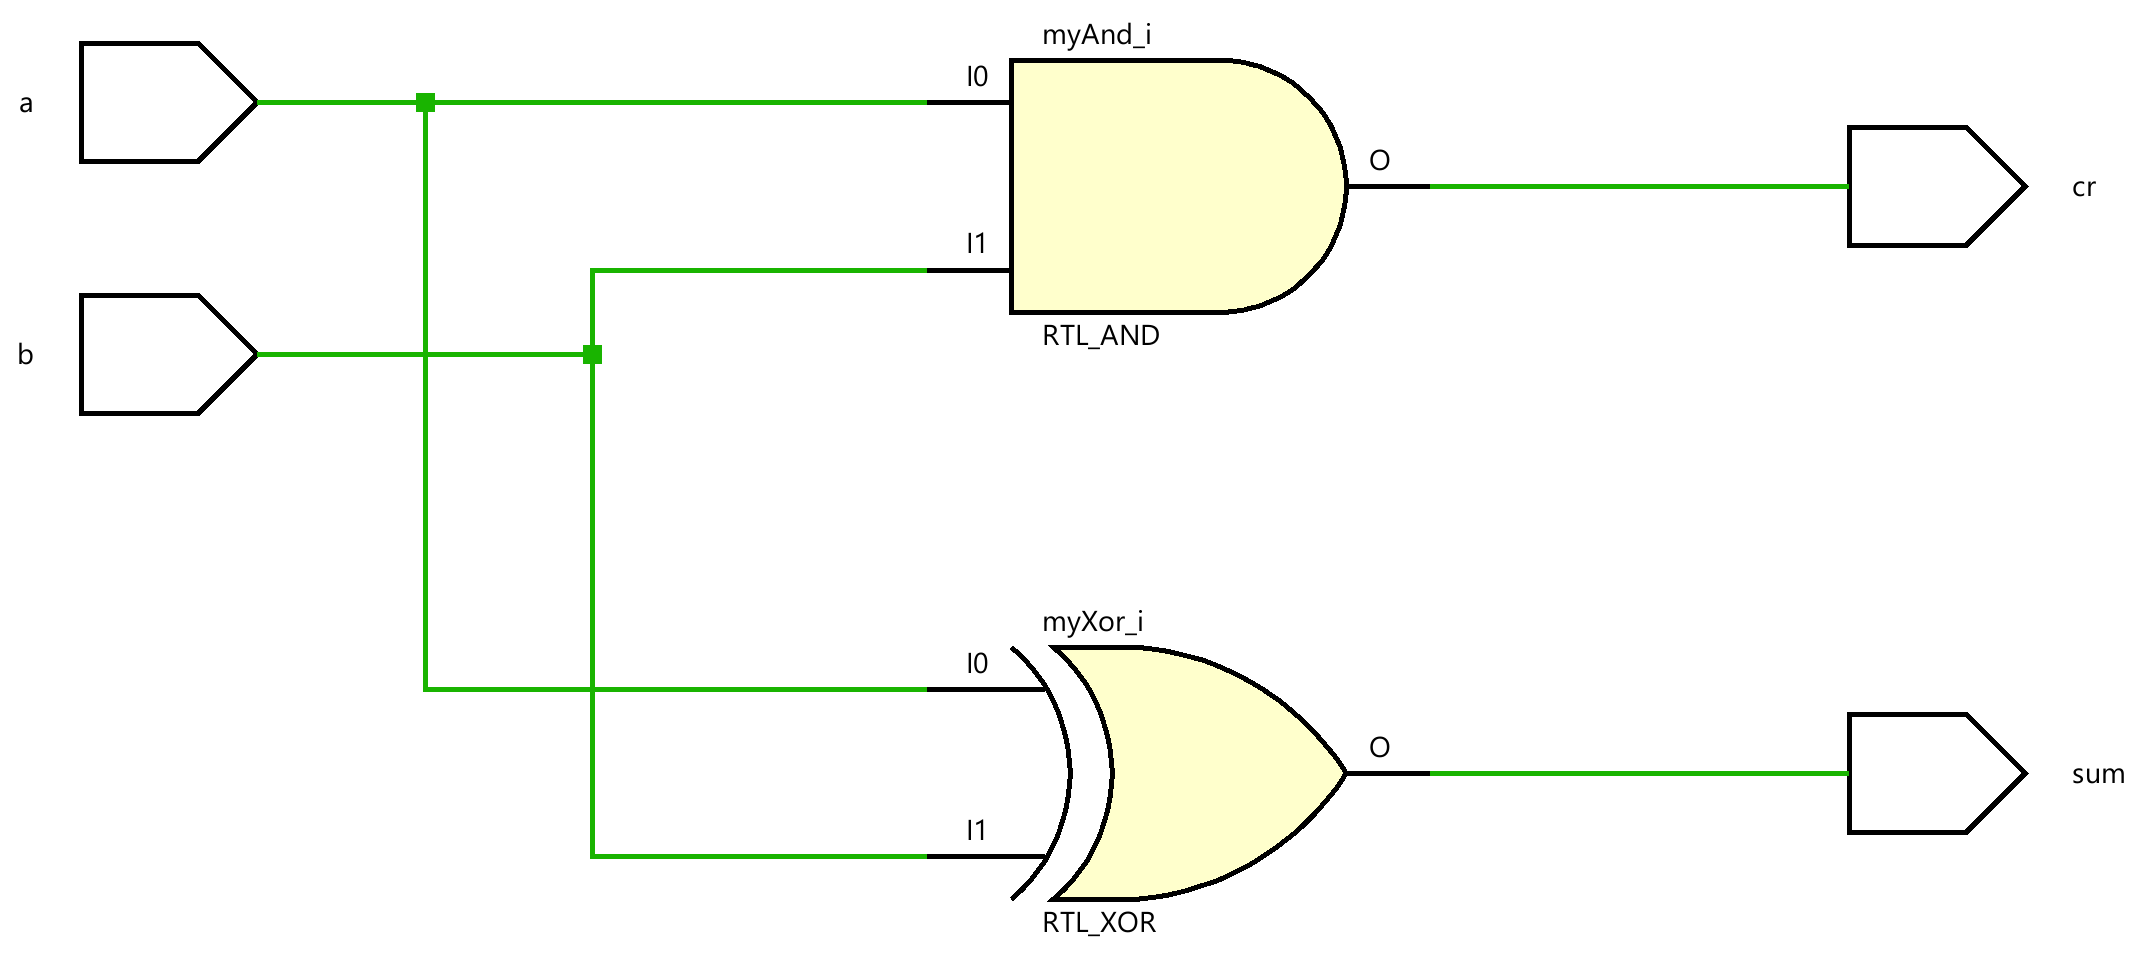
\includegraphics[width=\textwidth]{Latex/Images/halfAdder.png}
\end{center}
\concept{Implementation}:
\begin{itemize}
\item XOR gate for sum
\item AND gate for carry
\item Fundamental building block
\end{itemize}
\end{column}
\end{columns}
\end{frame}

\begin{frame}{Full Adder Circuit}
\begin{columns}
\begin{column}{0.6\textwidth}
\concept{Function}: Adds three bits (including carry-in)
\begin{itemize}
\item Inputs: $A$, $B$, $C_{in}$
\item Outputs: Sum ($S$), Carry-out ($C_{out}$)
\end{itemize}

\vspace{0.3cm}
\concept{Truth Table}:
\[
\begin{array}{|c|c|c|c|c|}
\hline
A & B & C_{in} & S & C_{out} \\
\hline
0 & 0 & 0 & 0 & 0 \\
0 & 0 & 1 & 1 & 0 \\
0 & 1 & 0 & 1 & 0 \\
0 & 1 & 1 & 0 & 1 \\
1 & 0 & 0 & 1 & 0 \\
1 & 0 & 1 & 0 & 1 \\
1 & 1 & 0 & 0 & 1 \\
1 & 1 & 1 & 1 & 1 \\
\hline
\end{array}
\]
\end{column}
\begin{column}{0.4\textwidth}
\begin{center}
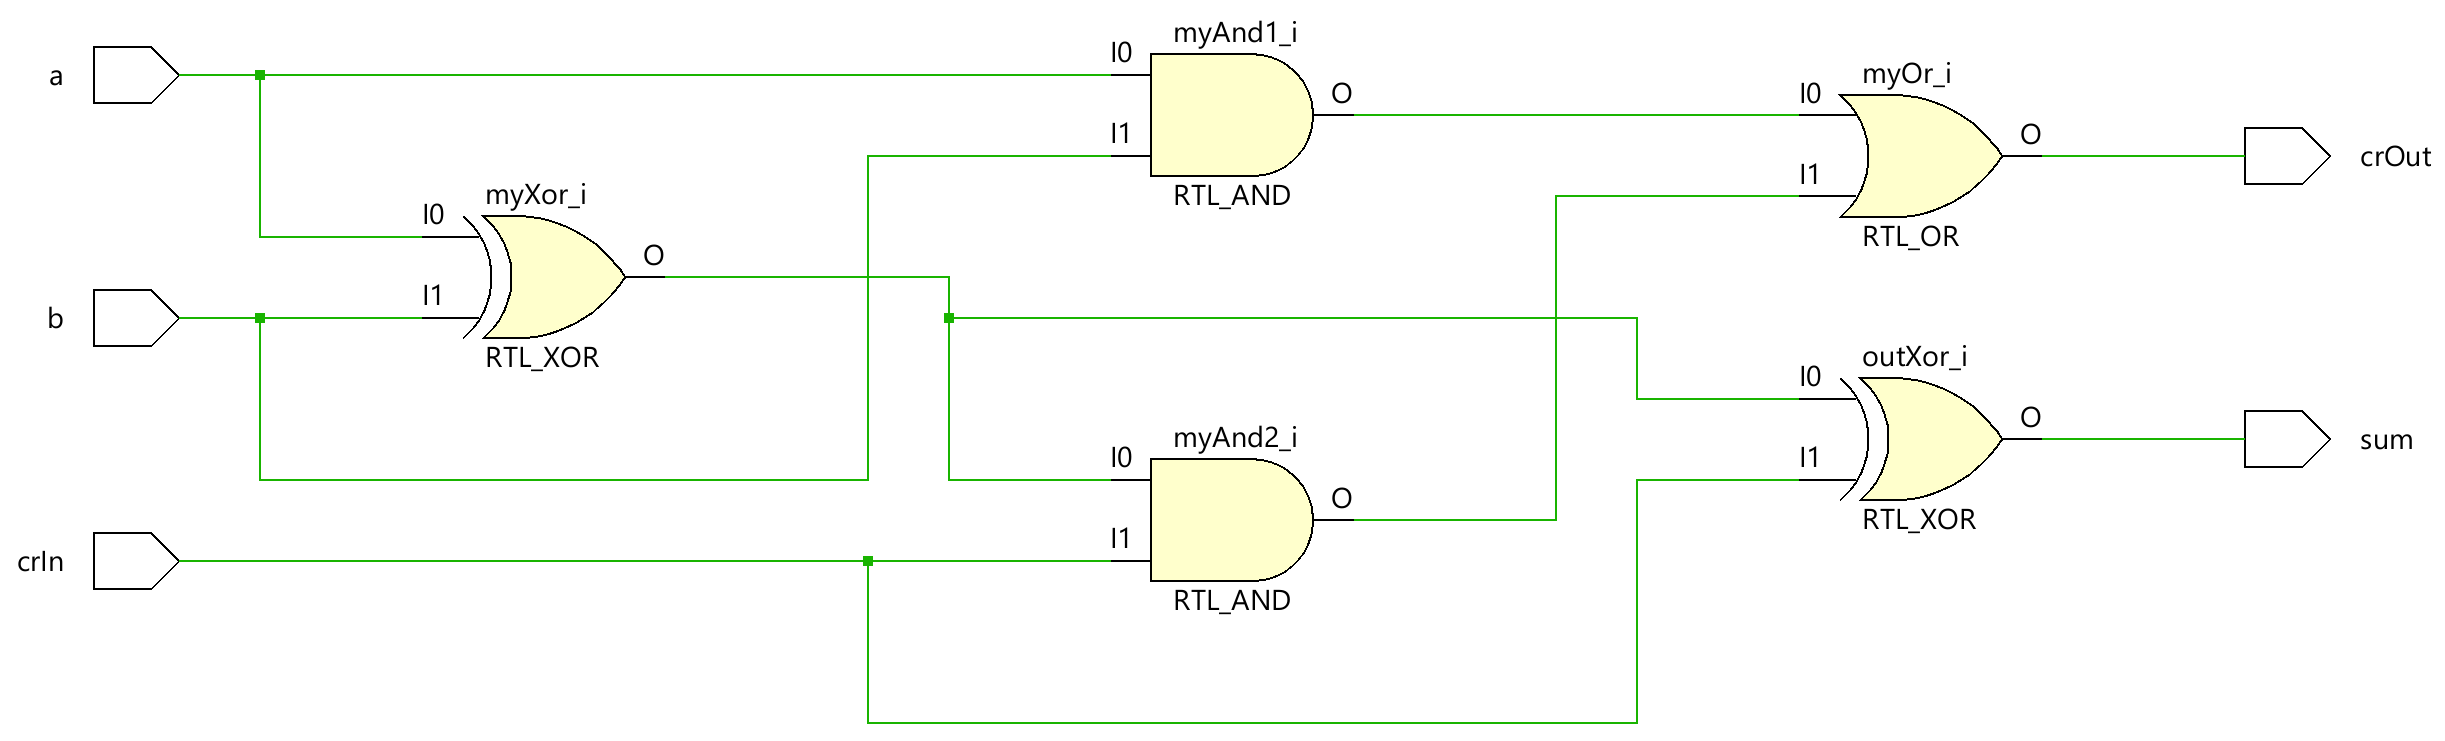
\includegraphics[width=\textwidth]{Latex/Images/fullAdder.png}
\end{center}
\concept{Boolean Expressions}:
\begin{align}
S &= A \oplus B \oplus C_{in}\\
C_{out} &= AB + C_{in}(A \oplus B)
\end{align}
\end{column}
\end{columns}
\end{frame}




\begin{frame}{Arithmetic Circuits}
\begin{itemize}
\item \concept{Multi-bit Adders}:
\begin{itemize}
\item Ripple-carry adder: Simple but slow
\item Carry-lookahead adder: Faster but more complex
\item Carry-select adder: Speed-area trade-off
\end{itemize}
\vspace{0.5cm}
\item \concept{Subtraction Circuits}:
\begin{itemize}
\item Two's complement representation
\item Subtraction as addition of complement
\item Overflow detection logic
\end{itemize}
\vspace{0.5cm}
\item \concept{Comparison Circuits}:
\begin{itemize}
\item Magnitude comparators
\item Equality detection
\item Greater-than/less-than logic
\end{itemize}
\end{itemize}
\end{frame}

% % subsection 8: Summary
% \subsection{Chapter Summary}

% \begin{frame}{Key Concepts Review}
% \begin{itemize}
% \item \concept{Boolean Algebra Foundations}:
% \begin{itemize}
% \item Mathematical basis for digital logic
% \item Laws and identities for simplification
% \item Historical development from Boole to Shannon
% \end{itemize}
% \vspace{0.3cm}
% \item \concept{Truth Tables and Logic Operations}:
% \begin{itemize}
% \item Systematic representation of logical functions
% \item Basic and advanced logic operations
% \item Circuit analysis and verification tool
% \end{itemize}
% \vspace{0.3cm}
% \item \concept{Combinational Circuit Design}:
% \begin{itemize}
% \item Systematic design methodology
% \item Building blocks: decoders, multiplexers, adders
% \item Optimization techniques and trade-offs
% \end{itemize}
% \end{itemize}
% \end{frame}

% \begin{frame}{Practical Applications}
% \begin{itemize}
% \item \concept{Digital System Building Blocks}:
% \begin{itemize}
% \item Foundation for all digital circuits
% \item Essential components in processors
% \item Building blocks for memory systems
% \end{itemize}
% \vspace{0.3cm}
% \item \concept{Design Methodology}:
% \begin{itemize}
% \item Specification to implementation flow
% \item Optimization for different goals
% \item Verification and testing approaches
% \end{itemize}
% \vspace{0.3cm}
% \item \concept{Technology Considerations}:
% \begin{itemize}
% \item Physical implementation constraints
% \item Performance optimization techniques
% \item Power and area trade-offs
% \end{itemize}
% \end{itemize}
% \end{frame}

% \begin{frame}{Connection to Higher-Order Systems}
% \begin{itemize}
% \item \concept{Foundation for 1-OS (Memory Circuits)}:
% \begin{itemize}
% \item Combinational logic + feedback = memory
% \item State storage and retention
% \item Clocking and synchronization
% \end{itemize}
% \vspace{0.3cm}
% \item \concept{Building Blocks for 2-OS (Automata)}:
% \begin{itemize}
% \item Control logic implementation
% \item State transition logic
% \item Output generation circuits
% \end{itemize}
% \vspace{0.3cm}
% \item \concept{Components of 3-OS (Processors)}:
% \begin{itemize}
% \item Arithmetic and logic units
% \item Instruction decoding logic
% \item Data path components
% \end{itemize}
% \end{itemize}
% \end{frame}

% % Questions slide
% \begin{frame}{Questions and Discussion}
% \begin{center}
% \Large
% Questions?

% \vspace{1cm}

% \normalsize
% \textbf{Discussion Topics:}
% \begin{itemize}
% \item How do Boolean laws enable circuit optimization?
% \item What are the trade-offs between different adder architectures?
% \item Why are NAND and NOR gates considered universal?
% \item How do combinational circuits form the foundation for sequential systems?
% \end{itemize}

% \vspace{0.5cm}
% \textbf{Next:} Chapter 2.9 - Memory Circuits: First-Order Systems (1-OS)
% \end{center}
% \end{frame}


